\documentclass[12pt]{article}
\usepackage{amsmath}
\usepackage{tikz}
\usepackage{enumerate}
\usepackage{algorithm2e}
\newcommand{\BigO}[1]{\ensuremath{\operatorname{O}\bigl(#1\bigr)}}
\newcommand{\BigOmega}{\ensuremath{\Omega}}
\usetikzlibrary{trees}


\begin{document}
\title{Chapter Three Assignment Solutions}
\author{CS310}
\date{October 15, 2013}
\maketitle
\newcounter{problem}
\setcounter{problem}{1}
\noindent \arabic{problem}.
Prove : $T(n) = T(n-1) + \Theta(n) = \Theta{n^2}$ by substitution

Suppose the guess, $T(n) = \Theta(n^2) $, is true. In order to prove that T(n) is $\Theta(n^2)$, one must show, through substitution, that there exist constants 
that make $c n^2$ both an upper and lower bound for the recurrence.

$ \frac{c_{1}}{2} (n-1)^2 - 1 \subset \Theta(n^2) $ so one can substitute it.

$T(n) <= \frac{c_{1}}{2} (n-1)^2 - 1 +  c_{1} n$

$T(n) <= \frac{c_{1}}{2} (n^2 - 2n + 1 - 1) + c_{1} n $

$T(n) <= \frac{c_{1}}{2} n^2 - c_{1} n + c_{1} n $

$T(n) <= \frac{c_{1}}{2} n^2   $

At this point, we have proven that $T(n) \subset \BigO{n^2}$

$T(n) >= \frac{c_{3}}{2} (n-1)^2 - 1 +  c_{3} n$

$T(n) >= \frac{c_{3}}{2} (n^2 - 2n + 1 - 1) + c_{3} n $

$T(n) >= \frac{c_{3}}{2} n^2 - c_{3} n + c_{3} n $

$T(n) >= \frac{c_{3}}{2} n^2   $

At this point, we have proven that $T(n) \subset \Omega(n^2) $ Since T(n) is also
$\subset \BigO{n^2}, T(n) \subset \Theta(n^2)$.
\stepcounter{problem}           

\vspace{10mm}
\noindent \arabic{problem}.

\stepcounter{problem}
\vspace{10mm}
\noindent \arabic{problem}.
Although Quicksort's asymptotic behavoir beats that of InsertionSort, real-world use cases may not be approximately asymptotic. If, as in the case of the bank,the average case invovles InsertionSort performing a constant number of swaps:

$T(n) = kT_{shift} + T(n-1)$    where  $k,T_{shift} \subset \Theta{1}$

$T(n) = \displaystyle\sum\limits_{i=1}^{n} \Theta{1}$

$T(n) \subset \Theta{n}$

Quicksort, on the other hand, will still take $\Theta{n * \log{n}}$ time.

\stepcounter{problem}

\vspace{10mm}
\noindent \arabic{problem}.
Since $ 0 < \alpha <= 1/2   $ , $1/2 <= (1 - \alpha) < 1 $

Because the recurrence terminates at n = 1, $ T(1) = T(\alpha^{h_{l}} * n) $ and $= T((1 - \alpha)^{h_{r}} * n) $ are expressions for the lefthand and righthand heights of the tree (where the left child of a node is $\alpha * parent$).  $ (1 - \alpha) > \alpha $ means that $ h_{r} > h_{l} $. Because any product, $\alpha^{n} * (1 - \alpha)^{m} $, is less than $(1- \alpha)^{n+m} $ and greater than $ \alpha^{n+m} $, the corresponding height would be between $h_{r}$ (the maximum) and $h_{l}$ (the minimum). 

$ T(1) = T(\alpha^{h_{min}} * n) $

$ k_{1} = k_{2} * \alpha^{h_{min}} * n $  where $ k_{1},k{2} \subset \Theta(1)$

$ \log_{\alpha}(k_{1} / (k_{2} * n)) = h_{min}  $

$ h_{min} = k_{3} * \frac{\log(1/n)} {\log(\alpha)} $ // by log arithmetic rules

$ h_{min} = k_{3} * - \frac{\log(n)} {\log(\alpha)} $ // by log arithmetic rules

\vspace{10 mm}
$ T(1) = T((1 - \alpha)^{h_{max}} * n) $

$ k_{5} = k_{4} * (1 - \alpha)^{h_{max}} * n $

$ \log_{(1 - \alpha)}(k_{1} / (k_{2} * n)) = h_{max}  $

$ h_{max} = k_{6} * \frac{\log(1/n)}{\log(1 - \alpha)}$ // by log arithmetic rules

$ h_{max} = k_{6} * - \frac{\log(n)} {\log(1 - \alpha)}  $ // by log arithmetic rules

\stepcounter{problem}
\vspace{10mm}
\noindent \arabic{problem}.

\stepcounter{problem}
\vspace{10mm}
\noindent \arabic{problem}.

\stepcounter{problem}
\vspace{10mm}
\noindent \arabic{problem}.
Definition of $\BigOmega(T_{2}): $ set of all $T_{1}$ $\lim_{n \to \infty} \frac{T_{1}(n)}{T_{2}(n)} > 0 $

In this case, $T_{2}(n) = \Theta(n * \log n) $.

Suppose randomized quicksort selects the maximum element of the unsorted subset for every iteration: $T_{1}(n) = T_{left} + T_{right} + \Theta(n) $ $T_{1}(n) = T(1) + T(n-1) + \Theta(n) $. In homework problem one, this recurrence was shown to be $\Theta(n^2)$. $\lim_{n \to \infty} \frac{\Theta(n^2)}{\Theta(n \log n)} > 0 $ is true so the runtime of randomized quicksort is big omega of n lg n.

\stepcounter{problem}
\vspace{10mm}
\noindent \arabic{problem}.

\stepcounter{problem}
\vspace{10mm}
\noindent \arabic{problem}.

Making quicksort tail recursive.
\begin{enumerate}[(a)]
\smallskip
\item The correctness of a sorting procedure is proven by demonstrating that the loop invariant is, in fact, invariant. The loop invariants for Quicksort are: 
\begin{enumerate}[I]
    \item If $ p <= k <= i$ , then $A[k] < A[i+1]$
    \item If $ i + 1 < k <= j - 1 $ , then $A[k] > A[i+1]$
\end{enumerate}

The postcondition of Partition is a list with the loop invariant met. If and only if, at recursive depth n, Partition has been called (n-1) times on the input size, will the loop invariant work towards a sorted list. In the following graph, the depth of a node represents the number of times Partition has been called
on the local input. The number in the node represents the sequential order of the call to Partition. If the value of every node is greater than the value of its parent, the correctness condition is met.

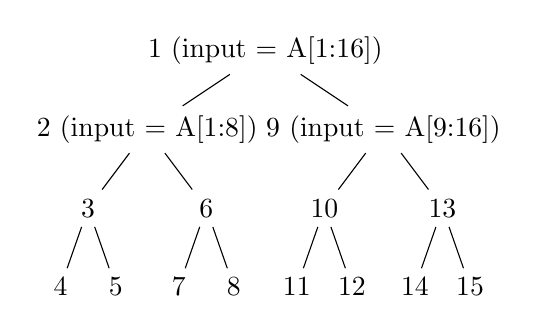
\begin{tikzpicture}[level distance=1.0cm,
    level 1/.style={sibling distance=3.0cm},
    level 2/.style={sibling distance=1.5cm},
    level 3/.style={sibling distance=0.7cm}]
    \node {1 (input = A[1:16])}
        child {node {2 (input = A[1:8])}
            child {node {3} 
                child {node {4}}
                child {node {5}}}
            child {node {6}
                child {node {7}}
                child {node {8}}}}
        child {node {9 (input = A[9:16])}
            child {node {10}
                child {node {11}}
                child {node {12}}}
            child {node {13}
                child {node {14}}
                child {node {15}}}
            };
\end{tikzpicture}

The correctness condition is met.

\smallskip
\item The stack depth will be $ \Theta(n) $ if the pivot is always the maximum element.

\smallskip
\item
\begin{algorithm}[H]
  \SetAlgoLined
  \While{p less than r}{
      q = Randomized-Partition(A,p,r)\;
      Tail-Recursive-Quicksort(A,lower,upper)\;
      p = q + 1\;
   } 
\end{algorithm}
This modification makes the worst case stack depth $ \Theta(lg n) $ because Randomized-Parition always puts a fraction on either side of the pivot. See the text for the definition of Randomized-Partition.
\end{enumerate}   
\end{document}            
